%!TEX root = ../dokumentation.tex

\chapter{Implementierung der Spielstrategie}

\section{Spielstrategien}
\subsection{Defensive Spielstrategie}
Bei der Defensiven Spielstrategie wird der Schläger nur auf einer geraden Linie parallel zum Tor bewegt. Bei dieser Strategie kann man grundsätzlich von 2 Situationen ausgehen. Die erste ist, der Puck bewegt sich auf den Roboter zu. In so einer Situation versucht der Roboter den Puck abzuwehren, erstmal ungeachtet ob der Puck sich überhaupt aufs Tor zu bewegt oder daran vorbeigehen würde. Bei der zweiten Situation bewegt sich der Puck vom Roboter weg. In diesem Fall sollte sich der Roboter zwischen dem Tor des Roboters und dem Puck positionieren und dem nächsten Angriff des Spielers zuvorzukommen.

Bei einer erweiterten Defensivstrategie könnte zum Beispiel zusätzlich überprüft werden ob der Puck überhaupt das Tor trifft oder in die Nähe des Tores kommt um unnötige Bewegungen zu vermeiden.

\subsection{offensive Spielstrategie}
Bei der Offensiven Strategie versucht der Roboter immer den Puck sofort zurückzuschlagen ohne an eine Verteidigung zu denken, frei nach dem Motto \enquote{Angriff ist die beste Verteidigung}. Dabei sollte angefangen werden, den Puck nur zurückzuschlagen ungeachtet der Richtung in welche dieser geschlagen wird. Sollte diese Taktik funktionieren, kann man dann ergänzen, dem Puck beim Zurückschlagen eine bestimme Richtung zu geben, damit der Roboter gezielter das gegnerische Tor trifft.

Später kann diese Strategie so erweitert werden, dass sich der Roboter nicht direkt auf den Puck zu bewegt, sondern sich vorher noch positioniert um eine bessere Angriffsposition zu haben.

\subsection{Defensive Spielstrategie mit offensiven Ansätzen}
Es wird weiterhin die selbe Taktik wie bei der rein defensiven Strategie genutzt. Zusätzlich wird ergänzt, das nach dem Blocken des Puckes, dieser mit der offensiven Strategie zurückgeschlagen wird.

\subsection{ausbalancierte Spielstrategie}
Bei der ausbalancierten Spielstrategie wird selbstständig vom Roboter entschieden, ob die Defensive oder die offensive Strategie verwendet wird. Bei der defensiven Strategie sollte die Verteidigungslinie auf einen Bereich unmittelbar vor dem Tor reduziert werden um unnötige Verteidigungsaktionen zu vermeiden.

\section{Strategieimplementierung}

Bei unserer Spielstrategie wird eine ausbalancierte Strategie verwendet. Um diese Strategie ausführen zu können, wurden vier unterschiedliche Befehle eingeführt. Diese kann man grundsätzlich in 2 Kategorien unterteilen, in defensive und offensive Befehle. 

Bei vieler dieser Funktionen und auch der Entscheidung wird eine Funktion zur Schnittpunktberechnung benutzt. Deshalb wird diese jetzt gleich vorab erklärt, wie sie funktioniert. Die Funktion für die Schnittpunktberechnung ist  im Quellcode~\ref{lst:Schnittpunktberechnung} auf Seite~\pageref{lst:Schnittpunktberechnung} zu sehen. Hier wird nur die Schnittpunkberechnung für eine X"~Linie, eine Gerade Parallel zur Y"~Achse, erläutert. Rückblickend betrachtet ist der Name vielleicht etwas ungünstig gewählt worden. Der Name entstand aber dadurch, dass alle X"~Werte auf dieser Linie den selben Wert haben.
Dieselbe Methode kann aber leicht umgeändert auch für Schnittpunkte mit einer Y"~Linie verwendet werden. Dieser Funktion können 2"~4 Parameter übergeben werden. Der erste Parameter ist der \textit{bag}. Der \textit{bag} enthält die Daten der Bilderkennung für die Puckposition, dessen Bewegungsrichtung und Geschwindigkeit. Der zweite Parameter ist xLine. Dies ist ein Wert zwischen 0 und 1, der den X"~Wert der zur Y"~Achse parallelen Linie im Bildkoordinatensystem enthält. Der dritte und vierte Parameter sind optional. Werden diese beiden Parameter übergeben, werden sie für die Schnittpunkberechnung als Ausgangswerte genutzt anstatt der Werte aus dem \textit{bag}. 

\begin{lstlisting}[caption= Python-Funktion für Schnittpunktberechnung, label=lst:Schnittpunktberechnung]
def CrossXLine(self,bag, xLine, startposition = None, direction = None):     
	if startposition == None:
		startposition = bag.puck.position
	if direction == None:
		direction = bag.puck.direction
	if direction[0] == 0:
		return None
	timeToCrossXLine = (xLine - startposition[0])/(direction[0] * bag.puck.velocity)
	yPosition = startposition[1] + timeToCrossXLine * direction[1] * bag.puck.velocity
	
	#Wenn der Puck ausserhalb der Spielfeldbegrenzung liegt, wird dieser vor dem zurueckgeben noch an der Spielfeldgranze gespiegelt
	koordinates = vector.mirror_point_into_field([xLine, yPosition])
	return (koordinates[0], koordinates[1], timeToCrossXLine)
\end{lstlisting}


\begin{wrapfigure}{r}{0pt}
	\vspace{-45pt}
	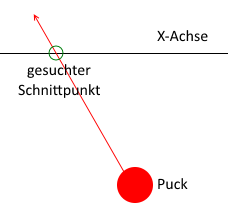
\includegraphics{Schnittpunktberechnung.png}
	\vspace{-15pt}
	\caption{Veranschaulichung der Schnitt"-punkt"-be"-rechnung}
	\vspace{-60pt}
	\label{img:Schnittpunktberechnung}
\end{wrapfigure}

Man kann mithilfe eines Punktes und eines Bewegungsvektors eine Gerade darstellen. Die Geradengleichung im 2-Dimensionalen Raum sieht in dann so aus: 

$\left(\begin{array}{c} x \\ y \end{array}\right) = \left(\begin{array}{c} x_P \\ y_P \end{array}\right) + k * \left(\begin{array}{c} x_R \\ y_R \end{array}\right)$. 

X und Y sind dabei die Koordinaten jeden beliebigen Punktes auf der Geraden. $X_P$ und $Y_P$ sind die Koordinaten eines beliebigen Punktes auf dieser Geraden. In unserem Fall ist dies die Position des Puckes. $X_R$ und $Y_R$ sind Teile des Richtungsvektors. Der Skalar k ist eine reelle Zahl, die den Richtungsvektor streckt oder staucht, um jeden beliebigen Punkt auf der Geraden zu erreichen. Im Bild~\ref{img:Schnittpunktberechnung} auf Seite~\pageref{img:Schnittpunktberechnung} ist dies nochmal grafisch dargestellt worden. Wir haben die Position des Puckes und die Bewegungsrichtung des Puckes. Wenn wir nun den Bewegungsvektor des Puckes entsprechend strecken oder stauchen, schneiden wir die gewünschte X"~Linie. Wir könnten nun für die gewünschte X"~Linie auch eine Geradengleichung aufstellen und dann die beiden Gleichungen in einem Gleichungssystem gleichsetzen, aber da wir bei der X"~Linie einen festen X"~Wert haben, überspringen wir diesen Teil einfach. Wir haben also nun folgende Gleichung, die es zu lösen gilt: 

$\left(\begin{array}{c} xLine \\ y_S \end{array}\right) = \left(\begin{array}{c} x_P \\ y_P \end{array}\right) + k * \left(\begin{array}{c} x_R \\ y_R \end{array}\right)$. 

Dies kann man nun in einem Gleichungssystem folgendermaßen dargestellt werden: 

$
\begin{array}{ccccccc}
xLine & = & x_P & + & k & * & x_R \\
y_S & = & y_P & + & k & * & y_R
\end{array}
$ 

\begin{wrapfigure}{R}{0pt}
	\vspace{-15pt}
	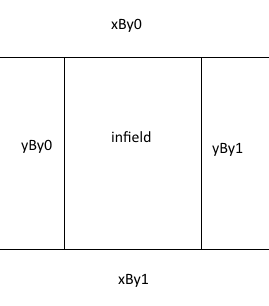
\includegraphics{Spiegelung_Quadranten.png}
	\vspace{-15pt}
	\caption{Quadranten bei der Spiegelung}
	\vspace{-15pt}
	\label{img:Quadranten}
\end{wrapfigure}

Wir haben somit die die Y"~Koordinate des Schnittpunktes $Y_S$ und den Skalar k als unbekannte Variablen. Die X"~Koordinate des Schnittpunktes \textit{xLine} wird als Variable an die Funktion übergeben und ist dadurch bekannt. Die erste Gleichung enthält somit nur die unbekannte k und kann nach k umgestellt werden. Wir erhalten damit die Gleichung: \\
$k = \dfrac{xLine - x_P}{x_R}$

Da in dieser Gleichung eine Division stattfindet, muss überprüft werden, ob der X"~Anteil des Bewegungsvektors $X_R$ ungleich null ist. Dies geschieht im Python Code in Zeile 6 und 7. Direction[0] ist dabei dieses $X_R$. Dies wird so dargestellt, da Vektoren in Python als Array behandelt werden. Vektoren sind somit 1-Dimensionale Array mit in unserem Fall 2 Werten. Der erste Wert, also direction[0] ist der X"~Anteil und der zweite Wert direction[1] ist der Y"~Anteil. Der Richtungsvektor der sich in dem Programm hinter bag.puck.direction verbirgt ist ein Einheitsvektor, das heißt dass dieser Vektor immer die Länge 1 hat. Deshalb multiplizieren wir zum Richtungsvektor in unserem Code noch die Geschwindigkeit auf. Dadurch erhalten wir einen Richtungsvektor, den der Puck in einer Sekunde beschreitet. Somit kann das errechnete k, oder wie wir es in unserem Code bezeichnen \textit{timeToCrossXLine}, auch für die benötigte Zeit genutzt werden, die später für die Angriffsstrategien wichtig ist. Anhand dieses Skalares kann man auch erkennen ob sich der Puck auf den Schnittpunkt zubewegt oder weg bewegt. Denn wenn $k>0$, dann bewegt sich der Puck auf die Schnittachse zu, ansonsten von ihr weg. 

Mit dem errechneten k, kann man nun auch die 2. Gleichung ausrechnen, um die Y"~Koordinate des Schnittpunktes zu erhalten. Dieser errechnete Wert kann aber unter Umständen außerhalb des Spielfeldes liegen und muss deshalb noch an den Banden in das Spielfeld gespiegelt werden. Dies übernimmt die Funktion \textit{mirror\_point\_into\_field}. Zu sehen im Quellcode~\ref{lst:Punktspiegelung} auf Seite~\pageref{lst:Punktspiegelung}. Diese Funktion nutzt dafür 2 andere Funktionen. Zum ersten die Funktion \textit{check\_for\_out\_of\_field} um den Quadranten zu berechnen in dem sich der Puck befindet. Dabei werden 5 Quadranten unterschieden, wie im Bild~\ref{img:Quadranten} auf Seite~\pageref{img:Quadranten} zu sehen ist. Der Quadrant 0, in unserem Quellcode \textit{infield} genannt, bedeutet, dass sich der Puck innerhalb des Spielfeldes befindet. Quadrant 1 und 2 bedeutet das sich der Puck in X"~Richtung außerhalb des Spielfeldes befindet. Wir haben diese Quadranten \textit{xBy0} und \textit{xBy1} genannt. Punkte in diesem Quadranten müssen an den X"~Achsen gespiegelt werden. Quadrant 3 und 4 bedeutet, dass sich der Puck in Y"~Richtung außerhalb des Spielfeldes befindet. Diese wurden respektabel \textit{yBy0} und \textit{yBy1} genannt. Diese Punkte werden an den Grenzen der Y"~Achsen gespiegelt. Die unterschiedliche Größe der Quadranten kommt durch die Reihenfolge der Berechnungen zu Stande. Die Spiegelung erfolgt im Bildkoordinatensystem bei dem die Koordinaten von (0/0) bis (1/1) gehen. Die Quadranten wurden deshalb nach der Spielfeldgrenzen benannt, an denen sie angrenzen und die Punkte in diesen Quadranten gespiegelt werden müssen.
Die zweite Funktion, die genutzt wird, ist die \textit{mirror\_point\_at\_border} Funktion. Dieser Funktion wird der zuvor berechnete Quadrant übergeben und berechnet dann den neuen gespiegelten Punkt. Um den neuen Punkt zu berechnen wird der Abstand des Punktes zur nahesten Spielfeldgrenze errechnet und dieser Abstand wird dann von der Spielfeldgrenze subtrahiert. Dies wird solange in einer Schleife wiederholt bis der Punkt im Spielfeld liegt.
\begin{lstlisting}[caption= Python-Funktion für Punktspiegelung, label=lst:Punktspiegelung]
def mirror_point_into_field(point):
    bordervalue = check_for_out_of_field(point)
    while bordervalue > 0:
	  point = mirror_point_at_border(point, bordervalue)
	  bordervalue = check_for_out_of_field(point)
    return point
   
def mirror_point_at_border(point, bordervalue):
    yPosition = point[1] 
    xPosition = point[0]
    if bordervalue == border.border.xBy0:
      xPosition = const.CONST.xBorderBy0 - (xPosition - const.CONST.xBorderBy0)
    if bordervalue == border.border.xBy1:
	  xPosition = const.CONST.xBorderBy1 - (xPosition - const.Const.xBorderBy1)
    if bordervalue == border.border.yBy0:
      yPosition = const.CONST.yBorderBy0 -(yPosition - const.CONST.yBorderBy0)
    if bordervalue == border.border.yBy1:
      yPosition = const.CONST.yBorderBy1 -(yPosition - const.CONST.yBorderBy1)
    return (xPosition, yPosition)
   
   
def check_for_out_of_field(point):
  if point[0] < const.CONST.xBorderBy0:
    return border.border.xBy0
  if point[0] > const.CONST.xBorderBy1:
    return border.border.xBy1
  if point[1] < const.CONST.yBorderBy0:
    return border.border.yBy0
  if point[1] > const.CONST.yBorderBy1:
    return border.border.yBy1
  return border.border.infield 
\end{lstlisting}



\subsection{defensive Strategien}
Der einfachste dieser Befehle ist die \enquote{\textit{Fahre die Home-Position an}}. Bei diesem Befehl platziert sich der Roboter direkt mittig vors Tor. In dieser Position ist es nur noch schwer möglich das Tor zu treffen, aber immer noch machbar. 

Der zweite Befehl ist der \textit{Verteidige} Befehl. Bei diesem Befehl bewegt sich der Roboter vor dem Tor auf die Bewegungsbahn des Puckes, damit dieser nicht in das Tor gelangt. Der Python Code für diesen Befehl sieht man im Quellcode~\ref{lst:defensivstrategie} auf Seite~\pageref{lst:defensivstrategie}.
\begin{lstlisting}[caption= python-funktion für Defensivstrategie, label=lst:defensivstrategie]
def defend(self, bag):
	koordinates = self.CrossXLine(bag, 0.0)
	robKoordinates = self.transformToRobotkoordinates(koordinates)
	#Position auf unmittelbar vors Tor beschraenken
	yMin = (const.CONST.RobYMax - const.CONST.Torgroesse) / 2.0
	yMax = (const.CONST.RobYMax + const.CONST.Torgroesse) / 2.0
	if robKoordinates[1] < yMin or robKoordinates[1] > yMax:
	  return None
	if abs(self.oldRobotKoordinates[1] - robKoordinates[1]) < const.CONST.minimumMovement:
	  return None
	self.lastMove = self.DEFEND
	#return explizit 0, da CrossXLine die 0 im Bildkoordinatensystem verwendet, die eine andere 0 als im Roboterkoordinatensystem ist
	return (0,robKoordinates[1])
\end{lstlisting}
Dazu wird zuerst der Schnittpunkt mit der Nulllinie der X-Achse berechnet. Diese liegt direkt an der Bande des Spielfeldes. Damit diese auch für den Roboter genutzt werden kann müssen die errechneten Koordinaten noch vom Bildkoordinatensystem in das Roboterkoordinatensystem umgerechnet werden. Um die Verteidigungsbewegung auch wirklich auszuführen, müssen noch 2 zusätzliche Kriterien erfüllt werden. Das erste Kriterium ist, das der Puck sich auch wirklich auf das Tor zu bewegt und nicht irgendwo neben dem Tor gegen die Bande prallt. Dies wird im Code in den Zeilen 5"~8 entschieden, indem zuerst die Torbegrenzungen  \textit{yMin} und \textit{yMax} berechnet werden. Sollte der errechnete Schnittpunkt außerhalb liegen, wird die Funktion abgebrochen. Sollte sich der Schläger bereits in einem gewissen Toleranzbereich vom errechneten Punkt befinden, soll sich der Roboter auch nicht erneut bewegen, da dieser dann für eine kurze Zeit nicht mehr reagieren kann. Dieser Toleranzbereich ist mit der Konstante \textit{minimumMovement} festgelegt und beträgt 25 mm. Sollten diese Fälle nicht eintreffen, merkt sich das Programm das es zuletzt diese Funktion ausgeführt hat und gibt die Koordinaten zu denen sich der Roboter bewegen soll zurück. Dabei wird für die X"~Koordinate explizit 0 verwendet, da die X"~Koordinate von der CrossXLine Funktion im Bildkoordinatensystem 0 ist, was nicht ganz exakt 0 im Roboterkoordinatensystem ist. Ansonsten gäbe es eine Verschiebung von etwa 3mm, die immer recht merkwürdig aussah wenn sie auftrat.


\subsection{offensive Strategien}
Es gibt 2 offensive Strategien. Die Strategie \textit{attack1} ist dabei die Vorbereitung auf den Angriff und \textit{attack2} ist Ausführung des Angriffes. Bei der Vorbereitung zum Angriff bewegt sich der Puck auf der Nulllinie der X"~Achse, so dass dieser dann nur noch eine Vorwärtsbewegung für den Angriff machen muss. Der Angriff ist dann quasi die Vorwärtsbewegung um den Puck zurückzuschlagen.
Den Sourcecode zu beiden Funktionen sieht man im Quellcode~\ref{lst:Offensivstrategien} auf Seite~\pageref{lst:Offensivstrategien}.
Der Funktion \textit{attack1} werden direkt die Koordinaten des errechneten Schnittpunktes übergeben. Es wird nur überprüft ob diese Koordinaten zu nah an den Außenbanden liegen um zu verhindern, dass der Roboter den Puck zwischen Bande und Schläger einquetscht. Sollte dies nicht der Fall sein, merkt sich das Programm das \textit{attack1} zuletzt ausgeführt wurde und gibt die Koordinaten zu denen sich der Roboter bewegen soll zurück.
Bei \textit{attack2} muss als erstes die aktuelle Position des Roboters vom Roboterkoordinatensystem ins Bildkoordinatensystem umgerechnet werden, da diese für die Schnittpunktberechnung benötigt wird. Für die Schnittpunktberechnung werden bei dieser Funktion je nach Situation unterschiedliche Schnittachsen verwendet. Sollte sich der Puck in einem spitzen Winkel von etwa 18$^\circ$ der Y"~Linie nähern, wird der Schnittpunkt zur X"~Linie etwa 20cm vor dem Tor berechnet. Sollte dieser Fall eintreffen, wird noch zusätzlich überprüft ob der Schlag nicht zu schräg wird, da dann unsere Berechnung zur benötigten Zeit des Schlages nicht mehr stimmt und um wieder zu verhindern. dass der Puck zwischen Bande und Schläger eingequetscht wird. Dieser Fall sollte zwar nicht eintreffen, da dieser vorher bereits abgefangen wird, ist aber aus Sicherheitsgründen hier immer noch enthalten. Sollte der Winkel zur Y"~Linie größer sein, wird der Schnittpunkt mit der Y"~Linie berechnet, wobei dann der Y"~Wert der aktuellen Roboterposition verwendet wird. Dies wird so gelöst, da die Berechnungen mit der Y"~Linie als Schnittachse genauer sind, da hier nur eine senkrechte Vorwärtsbewegung ausgeführt werden muss, anstatt einer leicht schrägen. Allerdings erhält man bei Spitzen Winkeln zur Y"~Linie häufig nicht nutzbare Werte dadurch. Sobald man den Schnittpunkt hat, wird noch überprüft ob dieser vom Roboter überhaupt erreicht werden kann. Dies sollte nur auftreten wenn der Puck während einer Pendelbewegung angegriffen wird und der Puck zu weit vom Roboter weg ist. Dies wird im Kapitel~\ref{sec:Strategieentscheidung} auf Seite~\pageref{sec:Strategieentscheidung} etwas genauer erklärt. Wenn der Roboter den errechneten Schnittpunkt in seiner Bewegungszeit mit Abweichung einer Framezeit erreichen kann, wird der Angriffsschlag ausgeführt, ansonsten wird gewartet bis er den Schnittpunkt in der errechneten Zeit erreichen kann.
\pagebreak
\begin{lstlisting}[caption= python-funktion für Offensivstrategien, label=lst:Offensivstrategien]
def attack1(self, robKoordinates):
	if robKoordinates[1] < const.CONST.durchmesserPuck:
	  return None
	if robKoordinates[1] > const.CONST.RobYMax - const.CONST.durchmesserPuck:
	  return None
	self.lastMove = self.ANGRIFF1
	return (0, robKoordinates[1])
    
def attack2(self, bag):
	#alte Roboterkoordinaten ins Bildsystem umrechnen
	y = (self.oldRobotKoordinates[1] + const.CONST.durchmesserSchlaeger / 2.0) / (const.CONST.tableWidth +  const.CONST.durchmesserSchlaeger)
	# sollte der Puck sich dem Schlaeger in einem Winkel kleiner 18 Grad naehern,
	# wird der schnittpunkt mit der x - Achse verwendet ansonsten der Schnittpunkt mit der y-Achse
	if bag.puck.direction[0] < -0.95:
	  koordinates = self.CrossXLine(bag, 0.18)
	  # Wenn der Schlag zu schraeg wird, Angriff abbrechen
	  if abs(koordinates[1] - y) > 0.2:
	    print("Angriff 2 abgebrochen")
	    return None
	else:
	  koordinates = self.CrossYLine(bag, y)	
	robKoordinates = self.transformToRobotkoordinates(koordinates)
	if not self.roboter.robCanReachPoint(robKoordinates):
	  return None
	if abs(self.calculateTimeToXPoint(robKoordinates) - koordinates[2]) < 1.0 / const.CONST.FPS:
	  self.lastMove = self.ANGRIFF2
	  return robKoordinates
	return None
\end{lstlisting}

\section{Strategieentscheidung}
\label{sec:Strategieentscheidung}
Für die Auswahl der richtigen Strategie haben wir einen komplexen Entscheidungsbaum entworfen, der auf verschiedene Parameter zurückgreift. Zu diesen Parametern zählen die aktuelle Position, die Bewegungsrichtung und Bewegungsgeschwindigkeit des Puckes, die zuletzt befahrene Position des Roboters und die zuletzt ausgeführte Aktion des Roboters. Im Bild~\ref{img:Entscheidungsbaum Strategieauswahl} auf Seite~\pageref{img:Entscheidungsbaum Strategieauswahl} sehen sie das Flussdiagramm dieses Entscheidungsbaumes. Wenn der Roboter als letzte Bewegung einen Angriff ausgeführt hat um den Puck zurück zu schlagen, steht in den meisten Fällen das Tor komplett frei. Um einen Konter entgegenzukommen, bewegt sich der Roboter anschließend sofort vors Tor. Denn so wird der Weg zum Verteidigen erheblich verkürzt. Wenn sich der Puck in der gegnerischen Hälfte befindet, werden nur defensive Strategien in Betracht gezogen, da sich der Roboter bei offensiven Strategien vom Tor entfernt und der Gegner die Bahn des Puckes immer noch beeinflussen kann. Sollte sich der Puck in der gegnerischen Hälfte vom Roboter wegbewegen, bewegt sich der Roboter zurück in die Homeposition um sich alle Möglichkeiten offen zu lassen, da der Puck vom Gegenspieler auf jeden Fall noch beeinflusst wird. Bewegt sich der Puck stattdessen schon auf den Roboter zu, soll dieser die \textit{Defend} Funktion aufrufen um einen möglichen Angriff bereits entgegenzuwirken.

Beim nächsten Schritt wird ermittelt ob der Puck auf der Spielfeldseite des Roboters pendelt. Als Pendeln haben wir festgelegt, wenn sich der Puck in einem Winkel kleiner 20$^\circ$ entlang der Y"~Achse bewegt. Dies ist der Fall, wenn der Betrag des normalisierten Bewegungsvektors in X"~Richtung kleiner als 0,35 ist, denn $\arccos 0,35 \approx 70^\circ$ in X"~Richtung, also etwa 20$^\circ$ in Y"~Richtung. Sollte sich der Puck in so einer Pendelbewegung befinden, fährt der Roboter mittig vors Tor oder wenn dies schon geschehen ist, macht der Roboter einen Angriffsschlag. Der Grund wieso der Roboter erst mittig vors Tor fährt ist folgender: Mit voll ausgestreckten Arm macht der Roboter eine Kreisförmige Bewegung, dadurch kann er unterschiedlich weit in das Spielfeld hineinreichen. Am Rand des Spielfeldes erreicht dieser eine Maximalreichweite von etwa 26cm, wohingegen er in der Mitte etwa 38cm schafft. Dadurch kann dieser fast 1,5x so weit reinreichen wie am Rande des Spielfeldes.
Aber diese 38 cm sind immer noch nur etwa 55\% seiner eigenen Spielfeldhälfte, wodurch dieser nicht immer den Puck erreichen kann und der Spieler warten muss, bis der Puck dann irgendwann mal auf seine eigene Hälfte zurück pendelt.

Sollten diese Entscheidungen nicht die richtigen gewesen sein, wird nun der Schnittpunkt mit einer X"~Linie, die sich etwa 20cm vor dem Tor befindet berechnet. Wenn die letzte Bewegung eine Vorbereitung auf den Angriff war, also \textit{attack1} ausgeführt wurde, wird überprüft ob die zuletzt berechnete Position nicht weiter als 2,5cm von der aktuell berechneten Position entfernt liegt. Diese 2,5cm sind die selbe Konstante \textit{minimumMovement}, wie sie auch im Defendalghorithmus auf Seite~\pageref{lst:defensivstrategie} verwendet wird. Sollte dies der Fall sein, wird die Funktion \textit{attack2} ausgeführt. Sollte als letztes nicht \textit{attack1} ausgeführt worden sein oder die neu berechnete Position weicht zu sehr von der alten ab, wird überprüft ob der Roboter mit eine Bewegung in Y"~Richtung und einer anschließenden Bewegung in X"~Richtung den Puck erreichen kann. Sollte die benötigte Zeit nicht ausreichen, also der Puck kommt vor dem Schläger an, wird die \textit{defend} Funktion ausgeführt. Sollte der Roboter aber genug Zeit haben, wird der Angriffsschlag mit der \textit{attack1} Funktion vorbereitet.

\begin{figure}[htbp]
	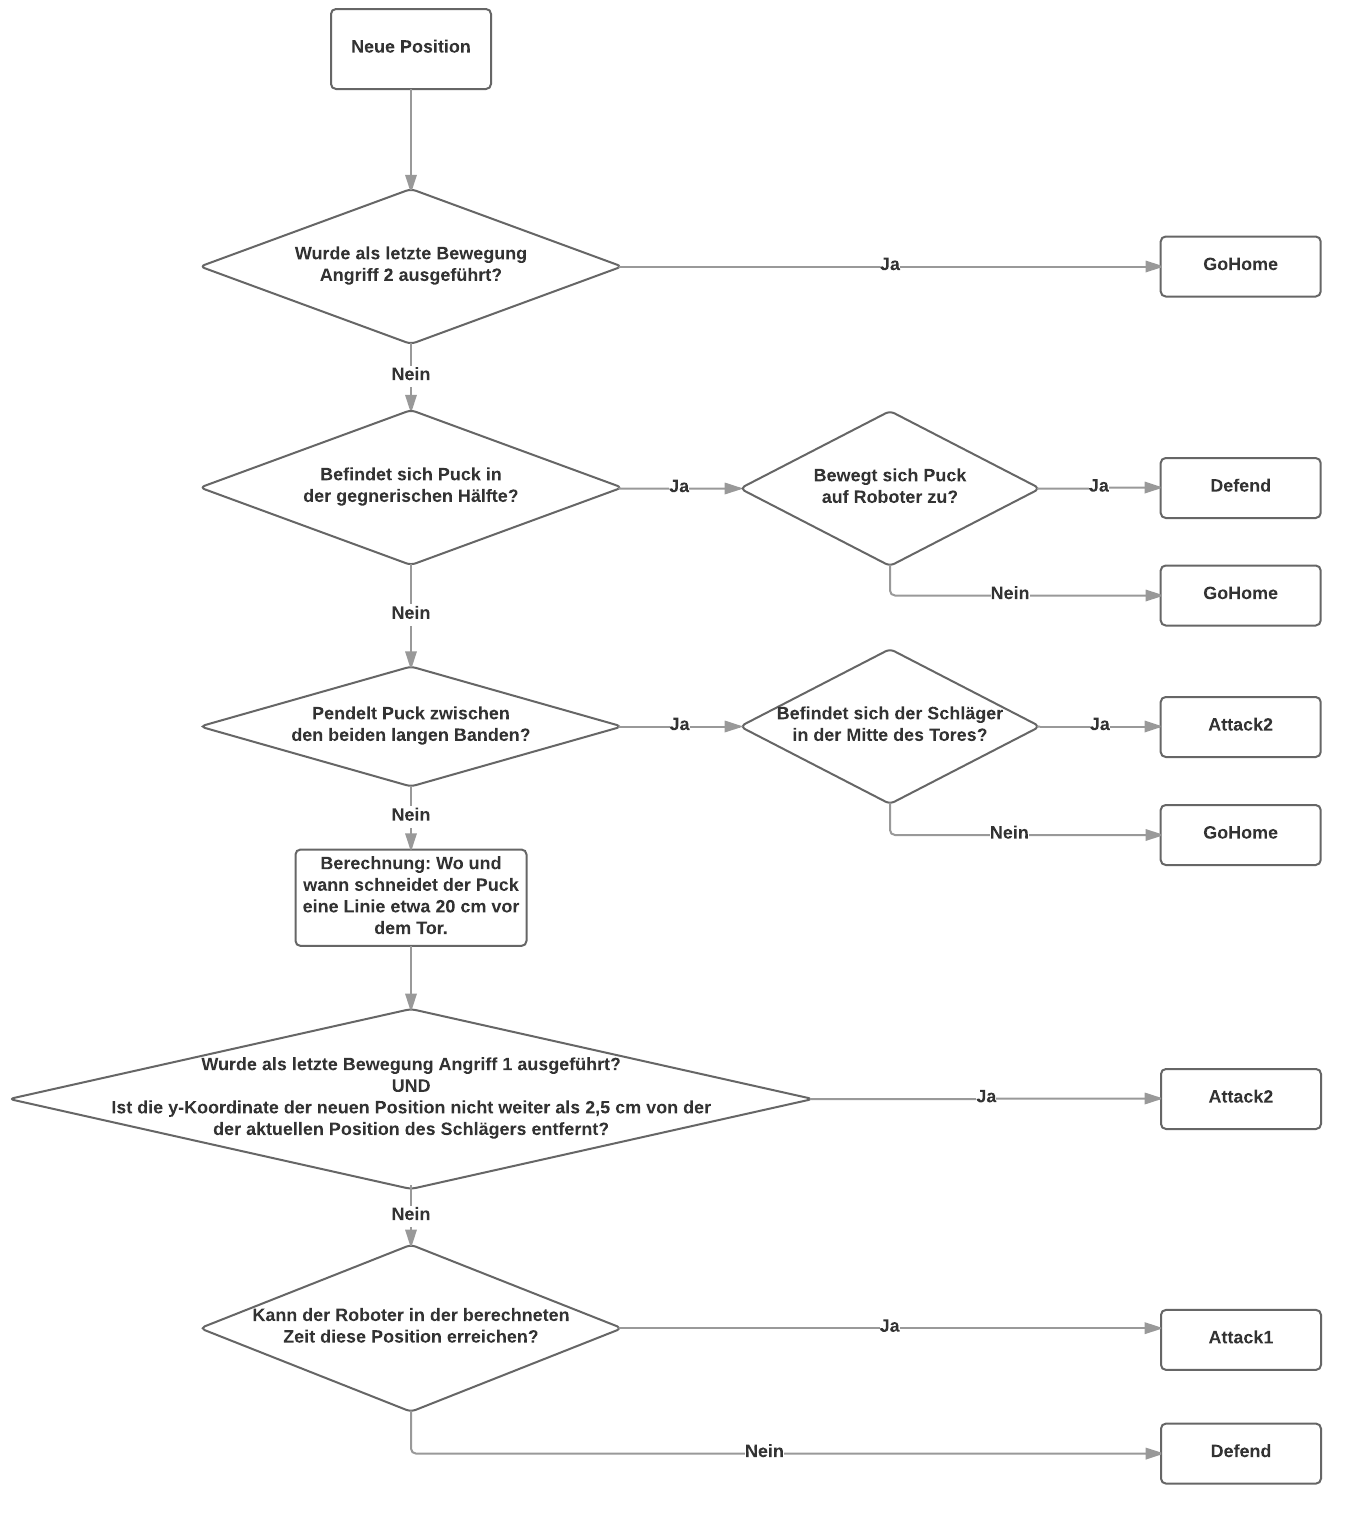
\includegraphics[width=\textwidth]{Stratigy_Decision1.png}
	\caption{Entscheidungsbaum für die Strategieauswahl}
	\label{img:Entscheidungsbaum Strategieauswahl}
\end{figure}